\documentclass[10pt,a4paper]{article}

\usepackage[margin=1.55cm]{geometry}
\usepackage{booktabs}
\usepackage{graphicx}
\usepackage{hyperref}
\usepackage{amsmath}
\usepackage{amssymb}
\usepackage{enumitem}
\usepackage{xcolor}
\usepackage{titlesec}
\usepackage{fancyhdr}

\setlength{\parindent}{0pt}
\setlength{\parskip}{3.5pt}
\setlength{\headheight}{19.7pt}
\setlist[itemize]{leftmargin=*, itemsep=1pt, topsep=2pt}
\titlespacing*{\section}{0pt}{0.4em}{0.25em}
\titlespacing*{\subsection}{0pt}{0.45em}{0.15em}
\titleformat{\section}{\large\bfseries}{\thesection}{0.5em}{}
\titleformat{\subsection}{\normalsize\bfseries}{\thesubsection}{0.5em}{}
\hypersetup{colorlinks=true, linkcolor=blue, urlcolor=blue}
\pagestyle{plain}
\fancyhf{}
\fancyhead[R]{\small Rawad Batous \\[-0.1em] rawad.batous2006@gmail.com}
\renewcommand{\headrulewidth}{0pt}

\newcommand{\code}[1]{\texttt{#1}}

\title{\vspace{-2.1em}\large European Power Fair Value: German Day-Ahead Forecasting and Prompt Curve Translation}
\author{}
\date{\vspace{-1.4em}}

\begin{document}
\maketitle
\thispagestyle{fancy}
\vspace{-3.0em}

\section*{Main Report}

\subsection*{1. What I Built, and Why This Is the Natural Shape}
The case study asks for a daily fair-value view that starts with public fundamentals and ends with something a power desk can actually discuss. The natural implementation is therefore not just a model; it is a chain of decisions: collect public ex-ante data, clean it without changing the information set, forecast the delivery window, measure uncertainty, aggregate into traded blocks, and compare the resulting fair value against a benchmark. My prototype follows exactly that chain for the German/Luxembourg day-ahead market.

Germany was chosen because it is a demanding market rather than a convenient one: high wind and solar penetration, frequent negative prices, strong intraday shape, and a volatile 2021--2025 regime. A model that works here has to learn more than a smooth daily seasonality. It has to respond to residual load, renewable forecast shape, weekdays, holidays, and the memory of recent prices. That makes Germany a good test of both the forecasting problem and the curve-translation problem.

The most important design choice is the information cutoff. A tradable forecast may use historical prices, calendar information, and forecasted load/wind/solar; it may not use future realised prices or future actual fundamentals. This sounds obvious, but it decides almost everything: the data source, the feature engineering, the validation scheme, and the difference between next-day and longer-period forecasts. The headline inputs are therefore ENTSO-E day-ahead forecast fundamentals, not realised fundamentals. In forecasting terminology, this is a tradable MOS-style setup, not a perfect-foresight oracle. It is a harder task, but it is the task a desk would actually face.

\subsection*{2. Data Quality and Time Handling}
The raw ingredients are ENTSO-E day-ahead prices plus load, solar, onshore wind, and offshore wind forecasts. The raw source files are not all delivered at the same frequency: some series arrive hourly and others can arrive at 15-minute granularity. The pipeline therefore first preserves the native responses, then parses and aggregates them to one hourly UTC table before modelling. These data satisfy the required price series plus multiple fundamental drivers, but more importantly they are aligned with the timing of the auction: load, wind, and solar enter as forecasts available before delivery.

The timestamp rule is deliberately strict: UTC is the technical key, German local time is an interpretation layer. All joins, validation windows, and lag construction happen on UTC timestamps. Local Europe/Berlin time is derived only for calendar behaviour and market blocks. This is what makes daylight-saving time manageable. A local delivery calendar has 23-hour and 25-hour days, but a UTC hourly key remains unique. Peakload/offpeak, however, must still be German local market time, so peakload is defined as weekday hours 08:00--20:00 Europe/Berlin.

The QA layer is not cosmetic. It checks missingness, duplicates, row coverage, obvious outliers, timestamp alignment, DST behaviour, and feature inventory. Missing forecast fundamentals are filled only from older same-hour values, repeatedly up to a week back if needed. That rule is intentionally simple: it can repair short source gaps, it is explainable, and it never copies future information backward. If a value still cannot be recovered from the past, the row is dropped before modelling. This gives a clean feature table while keeping the chronological story honest.

\subsection*{3. Forecast Setups: One Model Family Is Not Enough}
There are three forecast setups because the information set changes with the question being asked. For the hourly day-ahead setup, the model predicts the 24 hourly prices of one delivery day. It may use previous completed daily price curves such as d-1, d-2, d-3, and d-7, because those prices are known before forecasting tomorrow. This is the closest LEAR-style day-ahead task.

For the hourly-period setup, the model predicts hourly prices over a longer future period. Here, using yesterday-style price lags inside the period would silently become invalid: when forecasting a whole month from today, most ``yesterday'' prices inside that month do not exist yet. The safe implementation removes price-history features and relies on forecast fundamentals and calendar structure. The model becomes weaker, but the statement becomes defensible.

For the period-average setup, the target is changed directly: instead of forecasting every hour and averaging later, the model predicts baseload, peakload, and offpeak averages for the delivery period. This reduces the number of training observations, but it matches the curve object more directly. The three setups therefore answer three different business questions: tomorrow's hourly curve, a safe longer-period hourly view, and a direct period-average fair value.

Feature selection follows the same logic. LEAR and RANSAC-LASSO can use broad regularised feature sets; boosted trees and Theil-Sen worked better with compact, less collinear fundamental sets. The point is not that one feature set is universally best. The point is that each model/setup pair is given only the features that are valid for that forecasting question.

\subsection*{4. Validation and Model Evidence}
Validation uses rolling-origin splits: train on the previous 24 months, test the next month, then step forward one month. This produces 35 monthly folds from February 2023 through December 2025. Random K-fold validation would mix future and past regimes and is therefore not appropriate for electricity prices. The rolling design also mirrors live operation: retrain regularly, forecast the next window, score out-of-sample, move forward.

The baseline is deliberately meaningful: lag/mean behaviour depending on the target. It is not a straw man. The improved models are a LEAR-style regularised linear model, boosted trees, Theil-Sen, and RANSAC-LASSO. Metrics are kept focused: MAE, RMSE, bias, top-decile MAE, bottom-decile MAE, and scarcity-price MAE. MAE selects the model; tail metrics prevent a model from winning while failing exactly in stress hours.

\begin{table}[h]
\centering
\scriptsize
\begin{tabular}{llrrrrr}
\toprule
Setup & Model & MAE & RMSE & Bias & Top MAE & rMAE \\
\midrule
Hourly day-ahead & Baseline & 26.64 & 39.53 & +0.03 & 45.20 & 1.00 \\
Hourly day-ahead & LEAR LASSO & 16.50 & 26.69 & +0.96 & 31.18 & 0.62 \\
Hourly day-ahead & LEAR ElasticNet & 16.23 & 26.35 & +1.75 & 30.61 & 0.61 \\
Hourly day-ahead & Boosted tree & \textbf{15.28} & \textbf{23.94} & +2.17 & 30.28 & \textbf{0.57} \\
Hourly day-ahead & RANSAC-LASSO & 15.58 & 24.22 & -0.96 & \textbf{29.55} & 0.58 \\
\midrule
Hourly period & Baseline & 61.86 & 74.83 & +42.33 & 61.39 & 1.00 \\
Hourly period & Boosted tree & \textbf{28.30} & 40.14 & +16.06 & 52.99 & \textbf{0.46} \\
Hourly period & Theil-Sen & 29.85 & \textbf{39.57} & +17.42 & \textbf{52.50} & 0.48 \\
\midrule
Period average, 15d & Baseline & 18.16 & 21.25 & +0.40 & \textbf{25.61} & 1.00 \\
Period average, 15d & LEAR LASSO & \textbf{17.13} & \textbf{19.80} & +5.47 & 25.66 & \textbf{0.94} \\
\bottomrule
\end{tabular}
\caption{Selected rolling-validation results. Errors are in EUR/MWh. rMAE is MAE divided by the matching baseline MAE.}
\end{table}

The table has a clear story. For the true day-ahead task, every serious model beats the baseline by a large margin; the best boosted-tree run reaches 15.28 EUR/MWh MAE, about 43\% better than the baseline. LEAR and RANSAC-LASSO are close, which is reassuring because they come from different modelling assumptions. The longer-period hourly task is harder because unsafe price lags are removed, but the boosted tree and Theil-Sen still cut the baseline error by more than half. Direct 15-day period averages are closest to baseline: this is not a failure, but a statistical warning. Aggregating 15 days into one row per block gives far fewer samples, so I treat period-average modelling as a curve-relevant complement rather than the main evidence.

\subsection*{5. From Forecast to Curve View}
The curve translation is intentionally mechanical. Once hourly prices are predicted, baseload is the average over all hours, peakload is the German local weekday 08:00--20:00 average, and offpeak is the remaining hours. For direct period-average runs, those three block values are predicted directly. This is the bridge from day-ahead price modelling to prompt-curve language: the model does not output a vague ``price opinion'', it outputs block fair values.

The trading view compares forecast fair value with a benchmark. If a real forward or broker-screen price is available, it should be entered manually and treated as the benchmark. If not, the pipeline uses a documented proxy such as a trailing realised day-ahead average or same-month historical average. I do not call this a forward price; I call it a benchmark proxy. That distinction matters because the task explicitly allows not using forward data, but still asks for a method showing how the forecast would inform curve positioning.

The signal is band-driven, not point-forecast-driven. The model first creates an uncertainty band from out-of-sample validation residuals where possible. If the benchmark lies below the band, the view is long; if it lies above the band, the view is short; if it lies inside the band, the answer is neutral. If the benchmark is more than one full band width beyond the band edge, the signal becomes strong long or strong short. This prevents false precision. A 5 EUR/MWh edge is meaningful for a model with 3 EUR/MWh recent error; it is noise for a model with 25 EUR/MWh stress error. The generated report therefore gives fair value, benchmark, edge, signal, desk action, and invalidation logic together.

The invalidation logic is practical: resize or close the view if updated load/wind/solar forecasts move residual load materially, if outages or flows change the supply stack, if the model's recent error rises above validation error, or if executable market prices differ materially from the benchmark. In other words, the curve view is not a blind recommendation; it is a structured statement of model edge under known assumptions.

\begin{figure}[h]
\centering
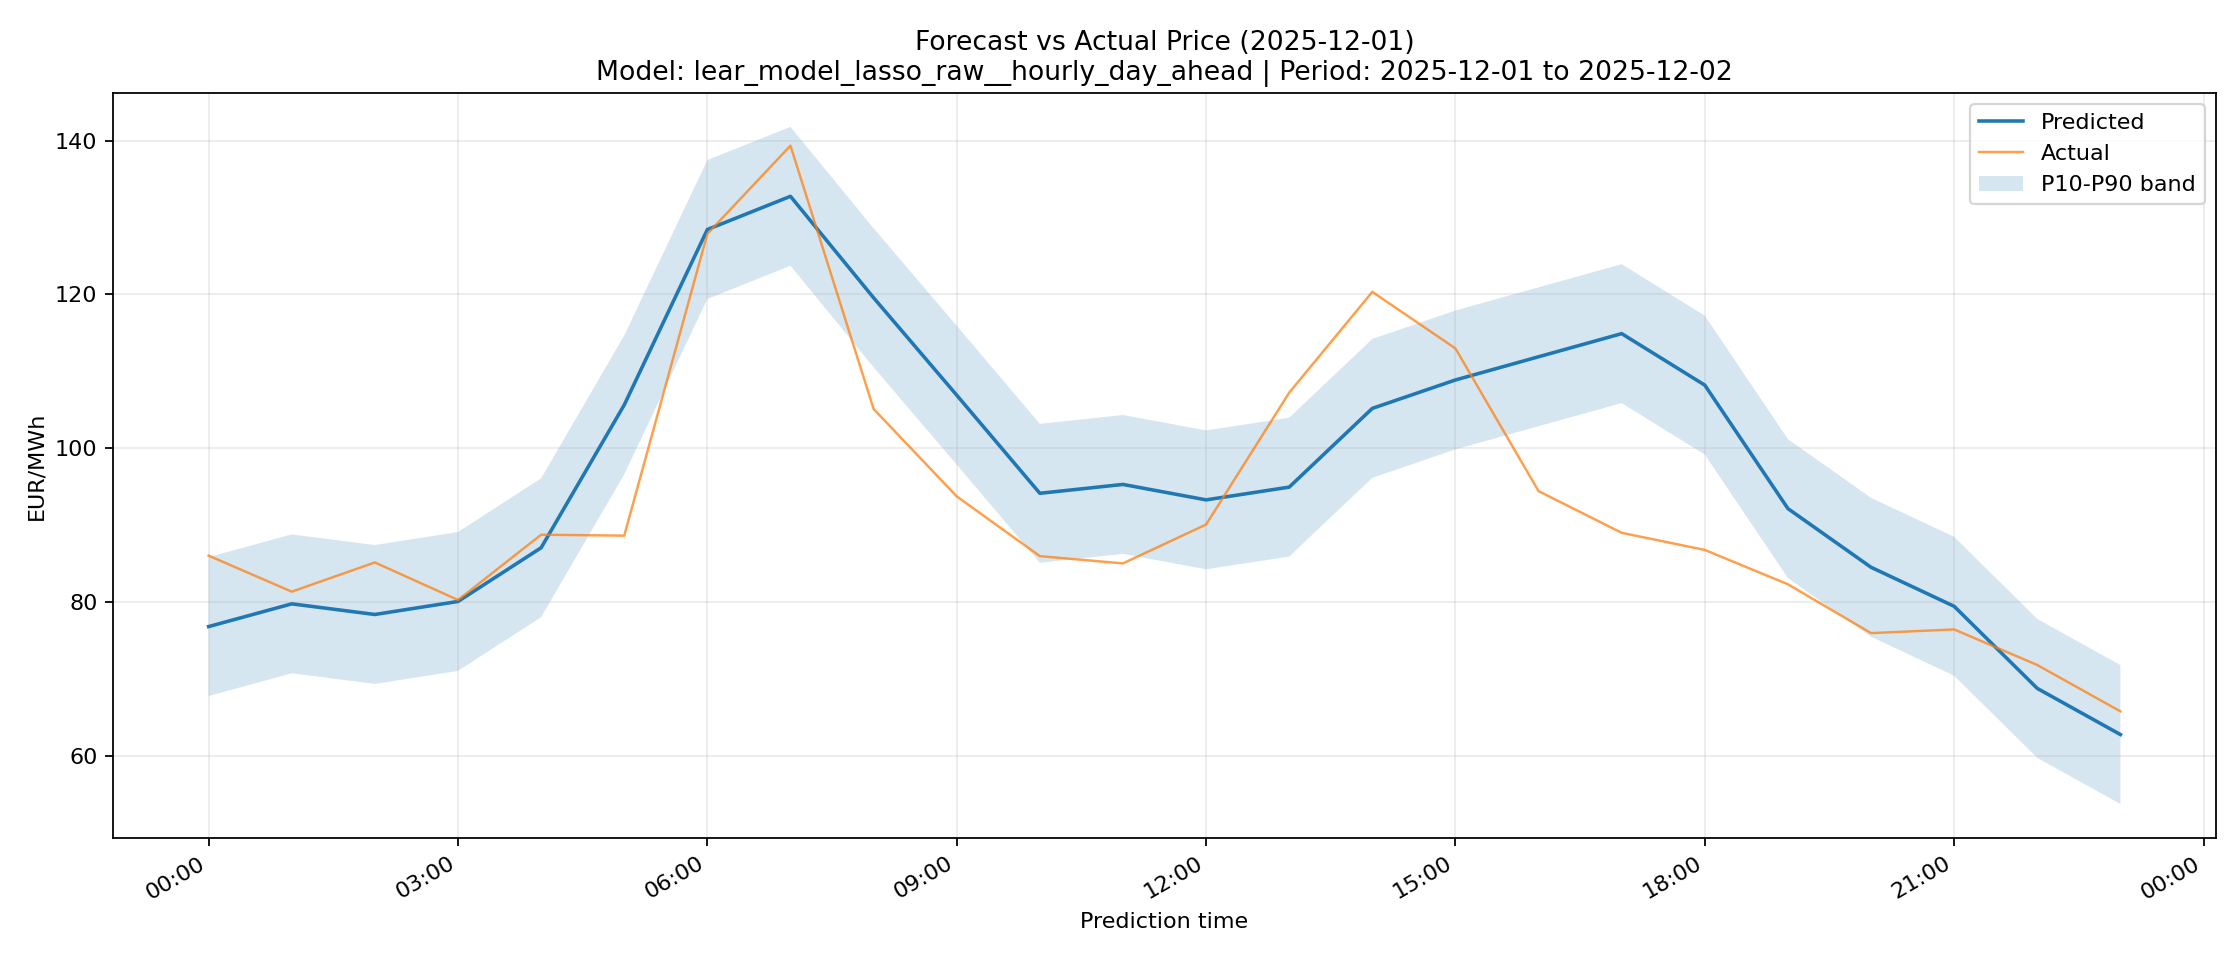
\includegraphics[width=0.47\linewidth]{outputs/germany_modelling_2021_2026/01-12-2025_02-12-2025/lear_model_lasso_raw__hourly_day_ahead/plots/forecast_actual_band.png}
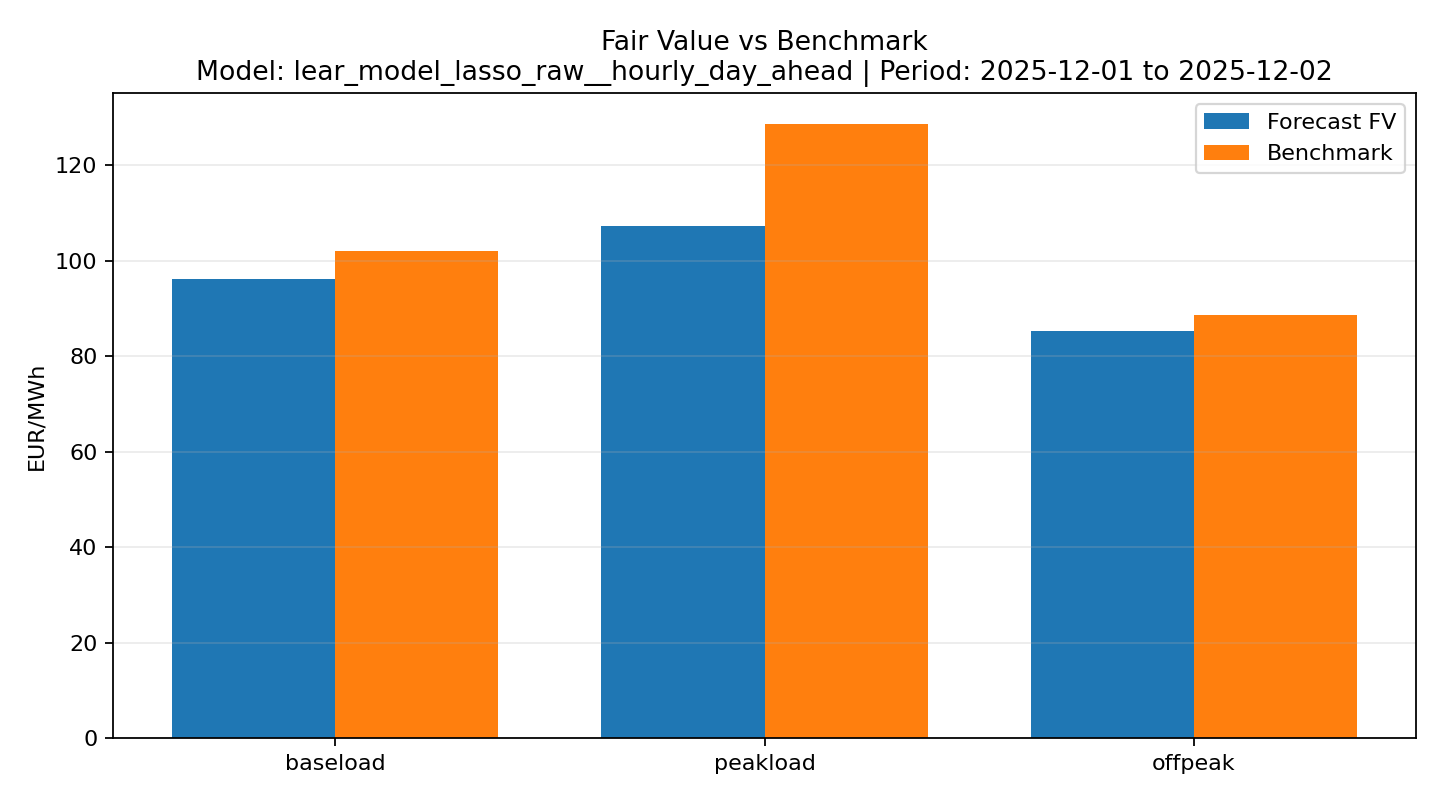
\includegraphics[width=0.47\linewidth]{outputs/germany_modelling_2021_2026/01-12-2025_02-12-2025/lear_model_lasso_raw__hourly_day_ahead/plots/fair_value_vs_benchmark.png}
\caption{One-day-ahead LEAR forecast band and block fair-value comparison generated by the forecast-view workflow.}
\end{figure}

\begin{figure}[h]
\centering
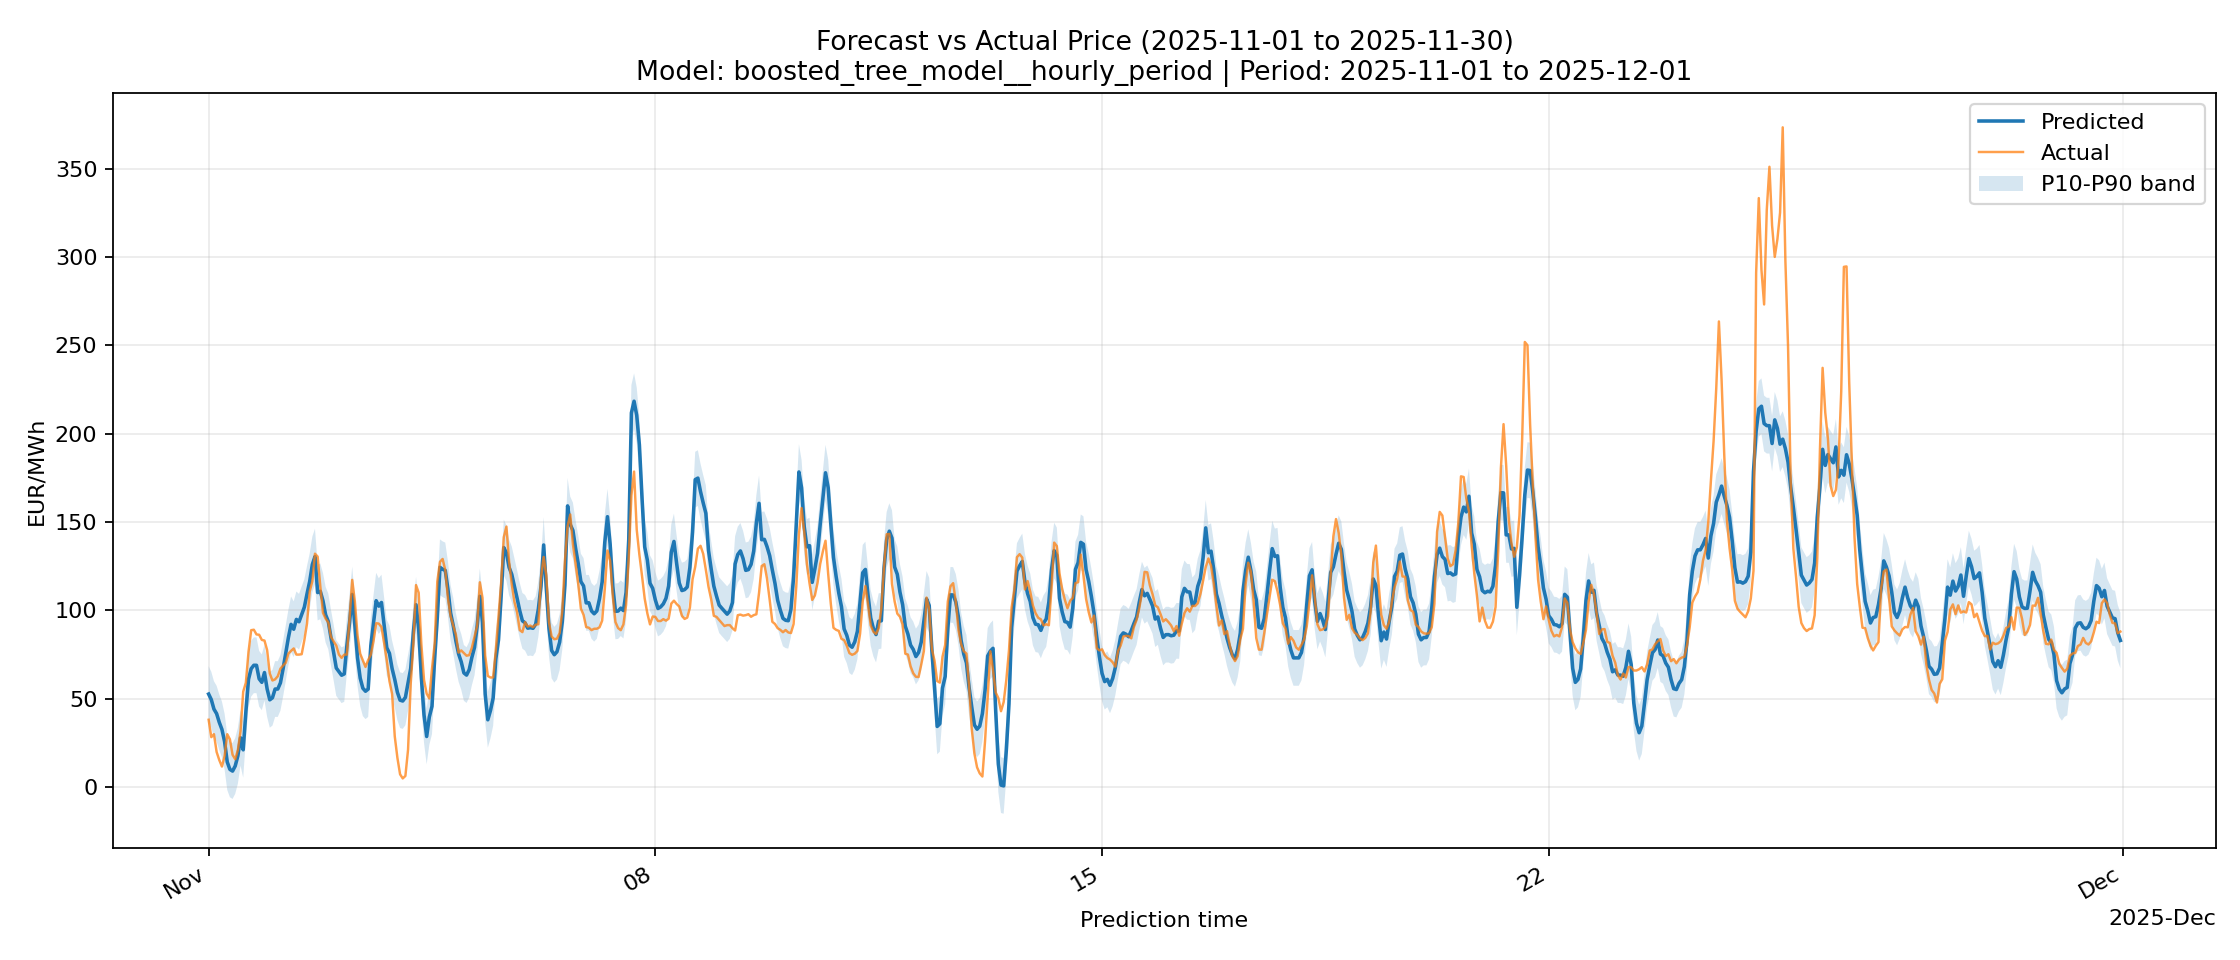
\includegraphics[width=0.47\linewidth]{outputs/germany_modelling_2021_2026/01-11-2025_01-12-2025/boosted_tree_model__hourly_period/plots/forecast_actual_band.png}
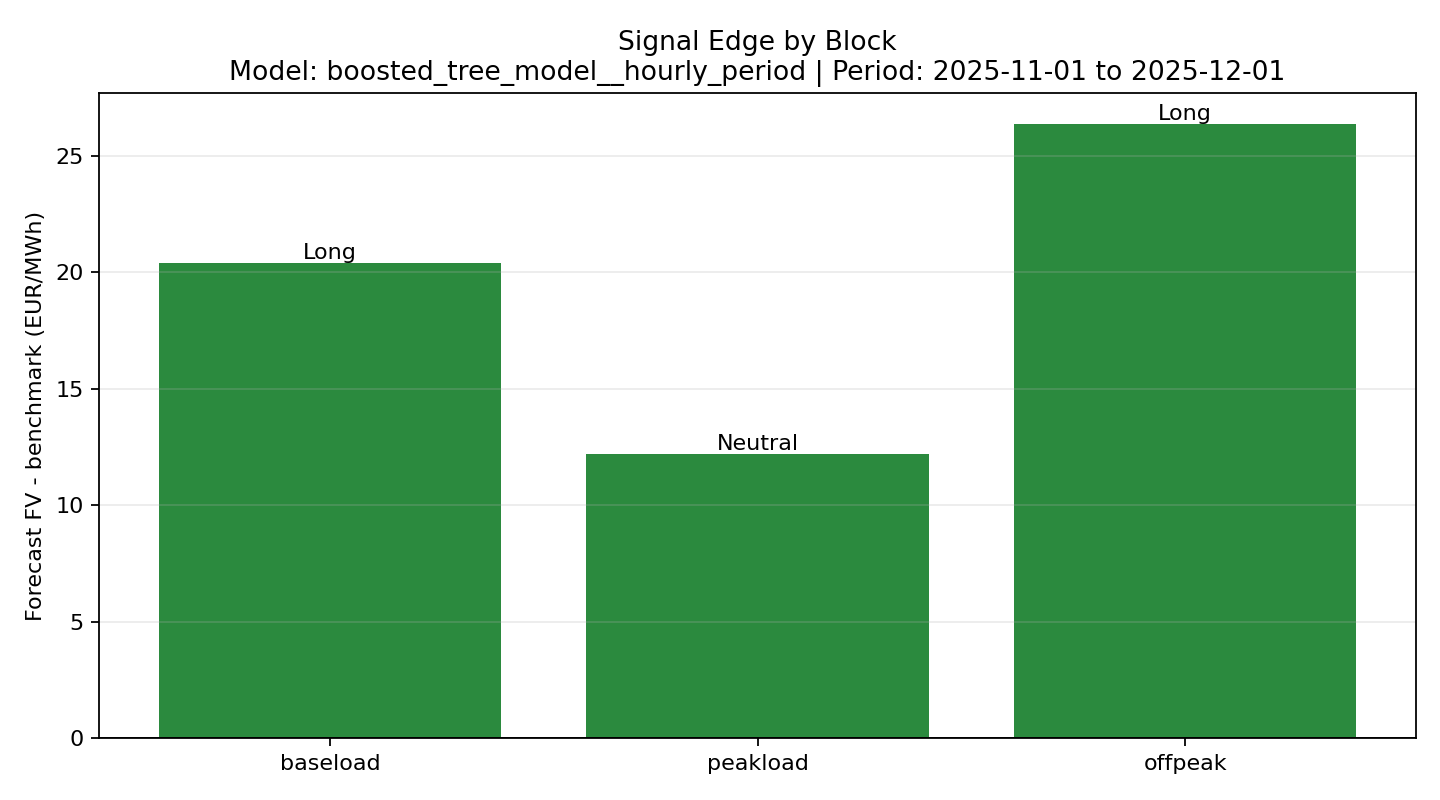
\includegraphics[width=0.47\linewidth]{outputs/germany_modelling_2021_2026/01-11-2025_01-12-2025/boosted_tree_model__hourly_period/plots/signal_by_block.png}
\caption{Longer-period boosted-tree prediction band and block signal view for the November 2025 delivery window.}
\end{figure}

\subsection*{6. Programmatic AI Component}
The AI step is deliberately narrow and auditable. It does not invent market analysis and it does not call a chat tool manually. It reads the computed curve-view summary, builds a constrained prompt that may only use the numbers in that table, calls the OpenAI API from code, and logs the prompt, output, and any failure. If the API key is absent or the API fails, a deterministic fallback commentary is produced from the same metrics, so the workflow still completes. This makes the LLM a controlled reporting accelerator rather than a source of hidden assumptions.

\subsection*{7. What This Prototype Proves}
The implementation proves the complete loop requested in the case study: public data ingestion, defensible QA, DST-safe alignment, leakage-aware forecasting, time-series validation, baseline comparison, stress metrics, forecast bands, prompt-curve translation, and a programmatic AI component. More importantly, the pieces fit together for one reason: the information set is respected all the way through. The model only sees what it could know; validation only tests unseen future windows; trading signals only fire when the edge clears uncertainty.

\subsection*{8. Desired Production Improvements}
The prototype deliberately prioritises information-set correctness and reproducibility. The first production improvement would be horizon-consistent fundamental forecasts. The longer-period hourly setup currently treats forecast load/wind/solar as if they are available for the whole requested future window. This is acceptable for a proof of concept, but a production system should use genuine multi-day, week-ahead, or month-ahead fundamental forecasts, or train separate models by forecast horizon.

The second improvement is richer market information. Public ENTSO-E load, wind, and solar are enough for the case-study minimum, but German power prices also react to gas, coal, EUA carbon, outages, hydro, and cross-border flows. Adding these drivers should improve period and curve forecasts more than repeatedly tuning the same model grid. A real traded forward or broker-screen price should also replace the realised-price proxy benchmark whenever available.

The third improvement is engineering scale. Rolling validation, hyperparameter grids, and window retraining are naturally parallelisable across folds, parameter settings, and sometimes delivery hours. Parallelisation would make boosted trees, RANSAC, and repeated operational retraining much faster. I would also add direct probabilistic models, such as quantile boosted trees, and an explicitly labelled oracle comparison using realised fundamentals to measure how much error comes from imperfect fundamental forecasts versus price-model error.

\newpage
\section*{Appendix: Mathematical Reasoning and Model Choices}

\subsection*{A. What the Literature Contributed}
The modelling path follows four ideas from the electricity-price and forecasting literature. First, the LEAR family of models, introduced by Ziel and used widely in the EPF literature, motivates a high-dimensional linear autoregressive model with exogenous fundamentals and separate hourly structure (\href{https://arxiv.org/abs/1509.01966}{Ziel, 2016}; \href{https://epftoolbox.readthedocs.io/en/latest/modules/lear_model.html}{epftoolbox}). Second, validation should be time-series based: Lago, De Ridder and De Schutter warn that random folds and weak baselines can produce overly optimistic electricity-price results (\href{https://arxiv.org/abs/2008.08004}{Lago et al., 2021}). Third, the distinction between realised fundamentals and forecast fundamentals is not cosmetic. This is the same practical distinction as MOS versus perfect-prog forecasting in meteorology: Marzban, Sandgathe and Kalnay discuss how MOS learns forecast-system biases while perfect-prog uses idealised realised/reanalysis inputs (\href{https://faculty.washington.edu/marzban/mos.pdf}{Marzban et al., 2006}). Fourth, price transformations can be useful for spikes and negative prices, so I tested the $\operatorname{asinh}$ idea motivated by Uniejewski and Weron (\href{https://www.mdpi.com/1996-1073/11/8/2039}{Uniejewski and Weron, 2018}) rather than assuming raw prices were automatically best.

The implementation is therefore not an attempt to make the most complicated model possible. It is an attempt to make the information flow correct: use public ex-ante fundamentals, validate chronologically, compare against a serious baseline, and only translate a forecast into a trade after attaching uncertainty.

\subsection*{B. Modelling Setup and Validity}
For a delivery hour $t$, let $y_t$ denote the realised day-ahead price and $X_t$ the features used to predict it. After training, the model is a fitted function $f_\theta$, where $\theta$ represents the learned parameters (linear coefficients, tree splits, or similar). If the forecast is made at time $T$, with available information $\mathcal{I}_T$, then validity means:
\[
  \hat{y}_t=f_\theta(X_t),
  \qquad
  X_t\subseteq\mathcal{I}_T.
\]
For a one-day-ahead delivery day $D$, valid features can include previous completed prices, the load/wind/solar forecasts for that day ($F_D$), and calendar variables for the target hour ($C_t$):
\[
  X_t\subseteq \{y_s:s<\min(D)\}\cup F_D\cup C_t,
  \qquad t\in D.
\]
For a longer future period $P$, the stricter condition is
\[
  X_t\cap\{y_s:s\in P\}=\emptyset,
  \qquad t\in P.
\]
This is the mathematical reason the project has different forecast setups. A feature that is valid for tomorrow can be invalid for a whole future month. Calling both cases by the same model name would hide leakage.

\subsection*{C. Targets: Hourly Forecasts and Period Fair Value}
For day-ahead forecasting the model predicts the full 24-hour vector
\[
  \hat{\mathbf{y}}_D=(\hat{y}_{D,00},\ldots,\hat{y}_{D,23}).
\]
From this vector the block fair value is
\[
  FV_B(P)=\frac{1}{|B|}\sum_{t\in B}\hat{y}_t,
\]
where $B$ can be baseload, peakload, or offpeak. This is Option A in the task statement: forecast hourly DA prices, then derive a curve-relevant block average.

The direct period-average setup is Option B:
\[
  z_{P,B}=\frac{1}{|B|}\sum_{t\in B}y_t,
  \qquad
  \hat{z}_{P,B}=g_\phi(W_{P,B}).
\]
Here $z_{P,B}$ is the realised average price of block $B$ in period $P$, $W_{P,B}$ is the period-level feature vector, and $\phi$ denotes the fitted parameters of the period-average model $g$. The target is already the delivery-period block average. It is closer to the traded object, but it has fewer training samples. That is why I keep both perspectives: hourly forecasts give more data and shape information; period-average models are cleaner for direct block views.

\subsection*{D. Transformations and Prediction Space}
The raw target is EUR/MWh. A model can either train directly on $y_t$ or on a transformation
\[
  u_t=H(y_t), \qquad \hat{u}_t=f_\theta(X_t), \qquad \hat{y}_t=H^{-1}(\hat{u}_t).
\]
The code supports the raw target and an $\operatorname{asinh}$ transform. The transform is useful in theory because power prices have spikes and negative values; $\log(y)$ is not safe for negative prices, while $\operatorname{asinh}(y)$ is defined everywhere. Motivated by Uniejewski and Weron's variance-stabilising discussion, I included it as an experimental target transform. In rolling validation on this dataset, however, it significantly worsened MAE compared with the raw target, so I removed it from the active final search. The important point is that transformations are treated as testable modelling choices, not as literature rules to apply blindly.

\subsection*{E. Rolling Validation and Metrics}
For fold $k$:
\[
  Train_k=[a_k,a_k+24m),\quad
  Test_k=[a_k+24m,a_k+25m),\quad
  a_{k+1}=a_k+1m.
\]
The main metrics are
\[
  MAE=\frac{1}{n}\sum_i |y_i-\hat{y}_i|,
  \qquad
  RMSE=\sqrt{\frac{1}{n}\sum_i (y_i-\hat{y}_i)^2},
\]
\[
  Bias=\frac{1}{n}\sum_i(\hat{y}_i-y_i).
\]
MAE is the headline because it is interpretable in EUR/MWh. RMSE punishes large mistakes more. Bias tells whether the model is systematically long or short. Top-decile, bottom-decile and scarcity-price MAE are tracked because the financially dangerous hours are not the average hours.

\subsection*{F. Bands, Coverage, and Why Coverage Matters}
A point forecast says where the model thinks the price is. A band says how uncertain that statement is. From out-of-sample validation residuals
\[
  e_t=y_t-\hat{y}_t
\]
the empirical P10--P90 offsets for local hour $h$ are
\[
  q_{0.1,h}=Q_{0.1}(\{e_t:hour(t)=h\}),
  \qquad
  q_{0.9,h}=Q_{0.9}(\{e_t:hour(t)=h\}).
\]
The forecast band is
\[
  [L_t,U_t]=[\hat{y}_t+q_{0.1,h},\ \hat{y}_t+q_{0.9,h}].
\]
Coverage measures calibration:
\[
  Coverage=\frac{1}{n}\sum_t\mathbf{1}\{L_t\le y_t\le U_t\}.
\]
For a P10--P90 band, the desired coverage is roughly 80\%. High coverage is desirable because it means the uncertainty band is honest. But coverage alone is not enough: a band can cover 100\% by being uselessly wide. This is why the band is used together with MAE and tail metrics.

\subsection*{G. Risk Estimation and Signal Rule}
For block $B$ and period $P$, let $Bench_B(P)$ be either a real curve price or a proxy benchmark. The forecast edge is
\[
  Edge_B(P)=FV_B(P)-Bench_B(P).
\]
The signal is not based on $Edge_B(P)$ alone. It is based on whether the benchmark clears the forecast band. Let the band width be
\[
  W_B(P)=U_B(P)-L_B(P).
\]
Then the implemented mapping is:
\[
\begin{cases}
\text{Strong long}, & L_B(P)-Bench_B(P)\ge W_B(P),\\
\text{Long}, & 0<L_B(P)-Bench_B(P)< W_B(P),\\
\text{Strong short}, & Bench_B(P)-U_B(P)\ge W_B(P),\\
\text{Short}, & 0<Bench_B(P)-U_B(P)< W_B(P),\\
\text{Neutral}, & L_B(P)\le Bench_B(P)\le U_B(P).
\end{cases}
\]
Here plain long/short are the weaker directional signals, while strong long/short mean the benchmark is at least one full band width outside the model's expected range. This is the risk discipline in the project. A positive edge is not automatically a long signal; it has to be large relative to the model's demonstrated uncertainty. When empirical bands are unavailable for a freshly retrained forward window, the fallback risk buffer is
\[
  FV_B(P)\pm\max(MAE,\ 0.5\cdot TailMetric).
\]

\subsection*{H. Why Different Models Want Different Features}
The LEAR/LASSO model can tolerate many correlated features because the LASSO penalty performs embedded feature selection:
\[
  \min_\beta \frac{1}{n}\sum_i(y_i-X_i^\top\beta)^2+\alpha\|\beta\|_1.
\]
If several variables explain the same signal, LASSO tends to keep a sparse subset. ElasticNet softens this by adding an $\ell_2$ component,
\[
  \alpha\left(\rho\|\beta\|_1+\frac{1-\rho}{2}\|\beta\|_2^2\right),
\]
which is useful when correlated features should share weight rather than one being selected arbitrarily. This is why broad LEAR feature sets are defensible.

Boosted trees behave differently. They do not need linear transformations and can learn nonlinear thresholds, but extra noisy or redundant columns can create unnecessary splits and increase runtime. Theil-Sen is even more sensitive: it is robust to outliers, but high-dimensional correlated features make the robust estimator unstable and expensive. RANSAC-LASSO combines sparse linear fitting with outlier rejection; it can help when spikes distort training, but it can also treat real scarcity events as outliers. Therefore the project does not force one universal feature set. The feature policy is model- and horizon-aware.

\subsection*{I. Short Model Map}
The baseline is the honest denominator: if a model cannot beat lag/mean behaviour, it is not useful. LEAR is the interpretable EPF workhorse: 24 regularised hourly regressions. Boosted trees are the nonlinear benchmark: they learn interactions such as residual load $\times$ hour without hand-coding them. Theil-Sen is a robust low-dimensional check. RANSAC-LASSO is a robust sparse check. This diversity is intentional: when different model families agree, the result is more credible; when they disagree, the disagreement points to where the data or feature assumptions need attention.

\subsection*{J. Submission Artifacts}
The submitted repository contains reproducible pipeline code, README instructions, requirements, generated QA output, validation tables, saved predictions, model metadata, figures, and AI prompt/output/failure logging. Any saved prediction file can be turned into the optional \code{submission.csv} by keeping the timestamp identifier and \code{y\_pred}.

\end{document}
